\documentclass{article}
\usepackage{graphicx}
\usepackage{color}
\usepackage{comment}
\usepackage{amssymb}
\usepackage{amsthm}

\newtheorem{definition}{Definition}

%%%%%%%%%%%%%%%%%%%%%%%%%%%%%%%%%%%%%%%%%%%%%%%%%%%%%%%%%%%%%%%%%%%%%

% Algorithms and pseudo code
\usepackage{verbatim}
\usepackage{algorithm}
\usepackage{algorithmicx}
\usepackage{algpseudocode}

% Graphics and display
\usepackage{float}
\usepackage{graphicx}
\usepackage{subfig}
\usepackage{enumerate}
\usepackage{url}
\usepackage{multirow}

% Math symbols and environments
\usepackage{amsmath}
\usepackage{amssymb}
\usepackage{stmaryrd} % \varcurlyvee


\usepackage{calc}%#%

% TikZ

\usepackage{tikz}
\usetikzlibrary{shapes,arrows}
\usetikzlibrary{positioning}

\definecolor{myyellow}{RGB}{255,255,150}
\definecolor{mylavender}{RGB}{125,249,255}
\definecolor{mygreen}{RGB}{144,238,14}
\definecolor{myred}{RGB}{255,0,0}

\newcommand\mytext[3][\scriptsize]{#2\\#1 #3}
\newcommand\mynode[4][]{%
  \node[mynode,#1,text width=\the\dimexpr#2cm] (#3) {\mytext{#3}{#4}}; 
}
\newcommand\mynot[4][]{%
  \node[mynot,#1,text width=\the\dimexpr#2cm] (#3) {\mytext{#3}{#4}}; 
}

\setcounter{secnumdepth}{4}

%%%%%%%%%%%%%%%%
%%%% Macros %%%%
%%%%%%%%%%%%%%%%

%%% Math
\newcommand{\nat}{\mathbb{N}}   % Natural numbers
\newcommand{\rat}{\mathbb{Q}}   % Rational numbers
\newcommand{\real}{\mathbb{R}}  % Real numbers
\newcommand{\runit}{[0, 1]}    % The real unit interval


% = with "hip." on the top, useful for indicating where a hypothesis comes in
\newcommand{\heq}{\stackrel{\text{\fontsize{3pt}{3pt}\selectfont hip.}}{=}}
% = because of the de Morgan laws.
\newcommand{\dmeq}{\stackrel{\text{\tiny{dM}}}{=}}


%%% Sets
\newcommand{\args}{\mathcal{A}} % Set of all arguments
\newcommand{\att}{\mathcal{R}}  % Set of all attacks
\newcommand{\valueset}{L}

%%% Votes on arguments
\newcommand{\varg}{V_{\args}}   % Function giving votes on arguments
\newcommand{\vargpro}[1]{\varg^+\left(#1\right)} % Pro votes on arguments
\newcommand{\vargcon}[1]{\varg^-\left(#1\right)} % Con votes on arguments

%%% Votes on attacks
\newcommand{\vatt}{V_{\att}}   % Function giving votes on attacks
\newcommand{\vattpro}[1]{\vatt^+\left(#1\right)} % Pro votes on attacks
\newcommand{\vattcon}[1]{\vatt^-\left(#1\right)} % Con votes on attacks

%%% Attack relations
% Attackers of a given argument
\newcommand{\attackers}[1]{\att^\text{-}\left(#1\right)} 
% Attackers of a given argument for the alternative framework F'
\newcommand{\altattackers}[1]{\att^{\prime\text{-}}\left(#1\right)}
% Ancestors of given argument according to the attack relation
\newcommand{\ancestors}[1]{\att^*\left(#1\right)} 

%%% Frameworks
\newcommand{\safid}{F}               % A single SAF, given by identifier
\newcommand{\safset}{\mathcal{F}}    % Set of all SAFs

\newcommand{\saf}{\safid = \safbody} % Framework id and respective tuple
\newcommand{\safbody}{\langle \args, \att, \varg, \vatt \rangle} % SAF tuple
% Alternative framework, same as \safbody but with ' everywhere ;)
\newcommand{\altsafbody}{\langle \args', \att', \varg', \vatt' \rangle} 

%%% Semantics
\newcommand{\semid}{\mathcal{S}}        % Semantic framework identifier
% Semantic framework tuple
\newcommand{\sembody}{\left\langle \valueset,\SAFand_1, \SAFand_2,\SAFor,\lnot,\tau \right\rangle}
\newcommand{\semdef}{\semid = \sembody}     % Semantic framework id and tuple
\newcommand{\semprod}[1]{\semid^\cdot_{#1}} % Product semantic framework
\newcommand{\semsub}{\semid^\text{-}}       % Subtraction semantic framework
\newcommand{\semmax}{\semid^\text{max}}     % Max semantic framework

\newcommand{\SAFand}{\curlywedge}     % Logical and for SAF equations 
\newcommand{\SAFor}{\curlyvee}        % Logical or for SAF equations
\DeclareMathOperator*{\SAFOr}{\bigcurlyvee} % Big or notation, works as \sum
                             %\varcurlyvee also works, but is smaller
\DeclareMathOperator*{\SAFAnd}{\bigcurlywedge} % Big and notation, works as \sum

\newcommand{\modelset}{\mathcal{M}}   % Set of all models


%#% old commands
\newcommand{\afit}{\textit{AF}}
\newcommand{\af}{\afit = \langle \args, \att \rangle}
\newcommand{\vote}{V}
\newcommand{\sem}{\mathcal{S}}

\newcommand{\ssv}{\mathcal{V}}
\newcommand{\tv}{\mathcal{T}}
\newcommand{\pv}{\mathcal{P}}
\newcommand{\xv}{\mathcal{X}}
\newcommand{\ev}{\mathcal{E}}

\newcommand{\safit}{F}

\newcommand{\tupd}{\curlywedge}
\newcommand{\tatt}{\curlyvee}
\newcommand{\Tatt}{\varcurlyvee}

\newcommand{\argarray}{\{x_1, ..., x_n\}}

\newcommand{\voteset}{\mathcal{V}}
\newcommand{\vpro}{\vote^+}
\newcommand{\vcon}{\vote^-}

%%% Mappings
\newcommand{\mapping}{\Phi}

%%%%%%%%%%%%%%%%%%%%%%%%%%%%%%%%%%%%%%%%%%%%%%%%%%%%%%%%%%%%%%%%%%%%%
%%%%%%%%%%%%%%%%%%%%%%%%%%%%%%%%%%%%%%%%%%%%%%%%%%%%%%%%%%%%%%%%%%%%%

\begin{document}

\title{Pointers for collaboration}

\maketitle

This document contains some pointers in order to extend the framework defined in \cite{leite2011social} \& \cite{eml2013esaf}.
\\
\section{The concept of support} %as an internal structure of the arguments}

%%{\color{red} }
%the intuitive idea
%%Embedding the concept of support relations in our system carries utmost importance.


%the objective:
In the current state, of our system there is no concept that could be directly mapped to the notion of support relations as in the works like \cite{DBLP:journals/ijis/AmgoudCLL08}. The only ways of realising indirect support in {\color{red}Social Abstract Argumentation} would be casting negative votes to the attackers of the supported argument, or in a similar sense to cast positive votes in favour of the attackers of the attackers{\color{red}, or by introducing some new arguments attacking to the original attackers}. Here the discussion is on if the system could benefit by having a more comprehensive mechanism with respect to the notion of support. 

{\color{red} 


Obviously, incorporating the notion of support is not a trivial matter and therefore one should carefully consider whether the realized method shows ingenuity and brings some clear advantage. 
%For instance, in \cite{gradinarg} authors try to capture the notion of support via \textit{paths}. 
For instance, the work in \cite{gradinarg} is based on the idea that indirect defenders are in fact supporters, and thus help strengthen an argument instead of minimising the damage done by an attacker. In this situation, it may happen that an argument attacked by more arguments may be stronger than one without certain attacks. The reason is that certain attackers may actually belong to a support path. In their work, a path from an argument to another is said to be an attack branch if its length is odd and a support branch if it is even. By emphasising the role of support branches in their global approach, it happens that argument $a$ is stronger in Figure \ref{subfig:wsup} than in Figure \ref{subfig:wosup}. This is because $a$ has one support and one attack branch in \ref{subfig:wsup}, and one attack branch and no support branch in \ref{subfig:wosup}. We do not share the same sentiment with this school of though, and actually argue the opposite. If one adds an attacker to argument $a$, then $a$ should not become stronger under any circumstances. It shouldn't matter whether there is a support branch: another attacker means further evidence that the attacked argument is not true. From this point of view, the best case scenario for $a$ would be for the new attacker to be defeated and $a$ maintaining its degree of truth. This illustrates two very different intuitions which do not seem trivially reducible to one another, if at all.

\begin{figure}[h!]
  \centering
  \subfloat[An argument with one attacker, without  support]{
    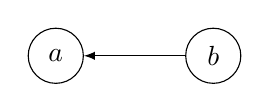
\begin{tikzpicture}[>=latex, auto]
  
    \tikzstyle{argument}=[draw, shape=circle, minimum size=7mm];
  
    \node [argument](a) at (0, 0){$a$};
    \node [argument](b) at (2, 0){$b$};
  
    \draw [->] (b) to (a);

    \end{tikzpicture}
    \label{subfig:wosup}
  } \hspace{1cm}
  \subfloat[Same argument with one support branch]{
    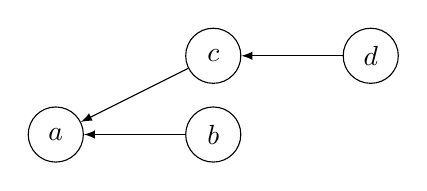
\begin{tikzpicture}[>=latex, auto]
  
    \tikzstyle{argument}=[draw, shape=circle, minimum size=7mm];
  
    \node [argument](a) at (0, 0){$a$};
    \node [argument](b) at (2, 0){$b$};
    \node [argument](c) at (2, 1){$c$};
    \node [argument](d) at (4, 1){$d$};

    \draw [->] (b) to (a);
    \draw [->] (c) to (a);
    \draw [->] (d) to (c);

    \end{tikzpicture}
    \label{subfig:wsup}
  }
  
  \caption{Addition of  a support branch}
  \label{fig:oops}
\end{figure}

There are also works(e.g. \cite{4}) which consider the attack and support relations as being independent and very much dual. But again it's doubtful whether the added complexity of considering a separate support relation worths its contribution to a social argumentation system. Suppose a simple example where $a$ supports $b$. The idea here is that if $a$ supports $b$, or in other words if $a$ is evidence for $b$, then to defeat $b$ one must first defeat $a$. Until there is no support or evidence for a given proposition, that proposition must be true. A set of supporting arguments can be seen as a conjunction, disjunction or mix of facts (the premises) that lead us to believe the conclusion (the argument which they support). The most obvious and direct solution for removing the support relation is to replace all these arguments with a new, structured argument. Its premises can be the supporting arguments (most logics trivially accommodate conjunctions, disjunctions or a mix as premises). Then, any argument that previously attacked a supporting argument can be considered an undercutting attack while any argument previously attacking the conclusion can be seen as a rebutting attack. Obviously, this is a simplified procedure, but nonetheless seems feasible. Once again, it is possible to remove the support relation from a framework, without altering its intended semantics. We do not believe the two relation notions have a symmetric nature, and  all in all we're not completely assured if the existing approaches are novel with respect to our application domain. 

}



%methodologies:
 {\color{red}A new and original methodology} to achieve this objective is an extension of the current framework with a notion of \emph{Pro-arguments}. In the sense that, instead of defining the counterpart of binary attack relations, the so-called support relations, we consider the new concept of Pro-arguments,  {\color{red}which would be of a somewhat different nature, more in line with structural parts of the arguments they defend rather than stand alone arguments. Therefore the correlation will not be realised via a binary relation, but Pro- arguments will simply be attached to their corresponding arguments as internal structures.} The social voting still will only take part on the arguments themselves, thus these structures should be interpreted as additional reasons to make users vote on that particular argument.

{\color{red} 

So briefly the method extends the framework of Social Abstract Argumentation \cite{eml2013esaf} in the following way: % with a set of \emph{PRO arguments}

\begin{definition}[Social argumentation frameworks]
A social argumentation framework is a 6-tuple $\langle \args, \mathcal{B}, \att, \mathcal{P}, \varg, \vatt \rangle$, where
\begin{itemize}
  \item $\mathcal{B}$ is the set of base-arguments,
  \item  $\mathcal{P}$ is the set of pro-arguments,
  \item $\args \subseteq \mathcal{B} \times 2^{\mathcal{P}}$  is the set of arguments,
  \item $\att \subseteq \args \times \args$ is a binary attack relation between arguments,
  \item $\varg : \args \to \nat \times \nat$ stores the crowd's pro and con votes for each argument.
  \item $\vatt : \att \to \nat \times \nat$ stores the crowd's pro and con votes for each attack.
%\item Rest of the notions follow the ESAF definition given in \cite{eml2013esaf}. 
\end{itemize}
\end{definition}

So as stated in the definition, now arguments are actually tuples which consist of a base-argument and a set of \textit{Pro-arguments}(which could be the empty set as well). Since the social voting  is still solely on arguments, the method does not force us to make any changes regarding the procedures of our system.

}

An alternative approach could be constructing a system without negative votes. Thus whenever a user is in favour of an argument, s/he will be casting a vote on the argument. So we maintain the notion of support realised as  a direct concept through votes. On the other hand if the user detests an argument, then s/he should find a counter argument to attack it, specify it by utilising the means of the system and then vote on the argument and the attack as well. {\color{red} This simply equates to only updating the mappings regarding the voting mechanisms of our framework. So formally, it follows as below:

\begin{definition}[Social argumentation frameworks]
A social argumentation framework is a 4-tuple $\langle \args, \att, \varg, \vatt \rangle$, where
\begin{itemize}
  \item $\mathcal{A}$ is the set of arguments,
  \item $\att \subseteq \args \times \args$ is a binary attack relation between arguments,
  \item $\varg : \args \to \nat$ stores the crowd's pro votes for each argument.
  \item $\vatt : \att \to \nat$ stores the crowd's pro votes for each attack.
\end{itemize}
\end{definition}

Since this approach is based on the idea of expelling the negative votes from the system, the mappings $\varg$, $\vatt$ only keep the positive votes for arguments and attacks, respectively. Of course now there is a need for modifying the vote aggregation functions as well since the set of parameters have changed. One can experiment with different choices of functions, perhaps the most obvious one being: $\tau(a) = v(a) / v_{max}$ where  $v_{max}$ stands for the maximum number of votes for an argument in the system. Thus only the argument(s) with the most number of votes in the framework would enjoy perfect social support.


}


%difficulties

{\color{red} 

In terms of difficulties,  reflecting all the info regarding the first approach at the same time poses a problem. We already have our conservations considering the comprehensibleness of the big systems in potential graphical representations. Indeed, this constitutes our main motivation for searching alternative graphical representations so the framework might prove to be more easily discernible by the users, and this idea is discussed in the following section.On top of the arguments and attack relations, adding \textit{Pro-arguments} in to the mix would possibly  make the GUI highly chaotic. Perhaps a good approach would be embedding the Pro-arguments into their associated argument. In the sense that one would only reveal them by clicking on the base argument, graphically in a similar way \textit{debategraph.org} displays the sub-relations of an argument. Moreover as mentioned earlier, even that we do not think the attack and support notions do not share a symmetric nature,  we may be asked by the user community to come up with a counter-part for the Pro-arguments.  In other words, a request for some internal structure for the arguments that contain criticism regarding the argument they're attached to. Another critique might be on the fact that each PRO argument changes the prior state of the argument.}
So even that the intended meaning of PRO arguments are to act as enhancers for the arguments they're associated to, indeed it could be possible that some users just won't share the same sentiment towards a particular argument anymore as a result of the addition of the PRO arguments. {\color{red} Thus users may either want to back up from supporting that argument. Additionally users may want to attack some Pro-argument without necessarily attacking to the argument it's associated to.

Regarding the second approach, it does not seem like serious technical difficulties would arise. This prospect is indeed plausible, since the latter approach is a simplistic state of our existing framework.} 
The most obvious potential criticism regarding this method  may point to the fact of the system lacking negative votes, as this had also been a major source of disconnect for a vast amount of Facebook users \cite{FBdislike}.


\section{Representing multi-dimensional dataset} 
%the intuitive idea
Displaying multivariate data of our framework via a multi-dimensional graph presents a challenge with respect to the ease of comprehension for the human users.

%methodologies:
An unorthodox yet interesting method that we may utilize, instead of using mere size and color changes of arguments, is the \textit{Chernoff faces}. They were first proposed by by Herman Chernoff \cite{Chernoff73} in 1973, as a way to represent multivariate data in a manner that is easily discernible by the human viewer.  The whole reasoning behind the use of Chernoff faces relies on the claim that humans are adept at face recognition and are able to notice reasonably acute changes in facial characteristics. The faces consist of two-dimensional line drawings that contain a variety of facial features. Moreover these facial features can be mapped to different dimensions in a multidimensional data set. The individual parts, such as eyes, ears, mouth and nose represent values of the variables by their shape, size, placement and orientation. In a similar sense, our approach would be mapping concepts from our framework such as  \textit{the social support of the argument, the social strength of the argument, the number of total votes that were casted on the argument and also the number of attacks that argument was being subjected to}, to distinct facial features. One notion that requires attention is that Chernoff faces handle each variable differently and because the features of the faces vary in perceived importance, the way in which variables are mapped to the features should be carefully chosen (e.g. eye size and eyebrow-slant was found to carry considerable weight compared to rest \cite{Morris00}).

%difficulties
In literature, there are mixed sentiments towards the validity of Chernoff faces. For instance in \cite{Morris00} authors claim that their experiments clearly depict that the use of Chernoff faces for information visualization does not take advantage of human pre-attentive visual processing, that Chernoff face feature perception is solely a serial process and not pre-attentive. Since the existing experiments do not seem to be decisively conclusive for neither schools of thought, perhaps the real value of Chernoff faces' use if our system can be best evaluated by carrying out our own tests.


\section{Voting schemes regarding negative votes}
%the intuitive idea
Our system does not have any assumptions on the intrinsic meaning of a \textit{negative vote}, however making a distinguish and handling the notions accordingly might prove to be fruitful.

%methodologies & difficulties:
Automated recognition of different schools of thought behind the negative votes casted by users is expected to be a hard problem. However if the classification can be made, it might be more plausible to use different operators in our system regarding their utilization. So in summary, the focus is on the question of whether a negative vote means the argument is badly spelled out, or simply the user does not like the {\color{red} conclusion of  the argument}. One methodology here can be rather than relying on automated mechanisms for capturing types, distinctly specifying the two types of negative votes and moreover their related operators. 

{\color{red} At first glance, this notion seems to be easily embeddable to our framework in the theoretical manner. It's important to note that here we assume the role of specifying the distinction of  different schemes of negative votes fall on the user community. So the idea is that as the framework architects, we would be supplying the users with a third option regarding the votes casted on the arguments. When this is the case, all needs to be done is updating mappings $\varg$ and $\vatt$ so that they can also record the additional negative vote type. Therefore the resulting framework would simply look as follows: 

\begin{definition}[Social argumentation frameworks]
A social argumentation framework is a 4-tuple $\langle \args, \att, \varg, \vatt \rangle$, where
\begin{itemize}
  \item $\mathcal{A}$ is the set of arguments,
  \item $\att \subseteq \args \times \args$ is a binary attack relation between arguments,
  \item $\varg : \args \to \nat \times \nat \times \nat$ stores the crowd's pro, con1 and con2 votes for each argument.
  \item $\vatt : \att \to \nat \times \nat \times \nat$ stores the crowd's pro,  con1 and con2 votes for each attack.
\end{itemize}
\end{definition}
}


Another point of debate worth mentioning is whether one can come up with a pure system where everyone has the same interpretation on what a negative vote is, or as mentioned earlier if some specific operator is better suited to a certain scheme of negative votes. In the case of the former scenario, we believe existing mechanisms of our current system for model evaluation are satisfactory, or least lay a strong foundation for future research.

{\color{red}
Even though we have stated that the former approach can be easily captured by the existing framework via small modifications, in reality the difficulty lies more in the operations and the semantics. The main question is how the additional scheme will be handled during the model evaluation. In the first section, we have discussed in detail the fact that we believe the attack and support relations do not correspond to each other in a dual-manner. Perhaps it should not be considered to the same extent, but still a similar discussion can be made with respect to the relation between positive and negative votes. Specifically, we think that a positive vote's reasoning is clear, simply meaning that the user agrees with the conclusion. However a negative vote could both stand for the dual of this notion, or simply represent a resentment regarding the way the argument was spelled out. All in all, adding this latter concept into the mix when dealing with concrete algebraic operations gives way to a lot of questions and thus proves to be an intriguing research opportunity.

Another challenge that transpires by the discussion of the different interpretations of votes is the concept of inconsistency with respect to the votes casted by a certain user. }Since the system constantly evolves, two arguments that a specific user was in favor of can all of a sudden be attacking to each other as a consequence of the introduction of some attack relation by another user. Moreover, if the interpretation of the votes is taken as an argument being well-structured or not, then it's perfectly plausible to cast "positive votes" on two mutually attacking arguments.

%difficulties(not so much)
Lastly, we may conclude that tests carried out via interacting with human users would be critical to see whether there is a dominant interpretation with respect to negative votes. 



\section{Bi-dimensional vote definition}
%the intuitive idea
In addition to the ratio of positive and negative votes, the total number of votes an argument has must be a significant parameter, when the system comes up with the final evaluation.

 In our existing system, the model of an argument is computed by roughly crunching  the number of positive and negative votes the argument has received into a single value in  $[0,1] \in \mathbb{R}$. There has been some early efforts in order to remedy this notion, scientifically for incorporating the effect of number of total votes into our vote aggregation function. For instance with the following definition:

%\newpage
\begin{definition}
[Vote Aggregation]A vote aggregation function is any function
$\tau:
\mathbb{N} \times \mathbb{N} \times \mathbb{N}
\rightarrow\lbrack0,1]$ such that $v_{max}\geq0$
\[
\tau\left(  v^{+},v^{-}, v_{max}\right)  =\left\{
\begin{array}
[c]{lll}
0 &  & v_{max}=0\\
\frac{v^{+}}{v^{+}+v^{-}+\frac{1}{v_{max}}} &  & \text{otherwise}
\end{array}
\right.
\]

where $v_{max}$ stands for the maximum number of votes for an argument in the system.
\end{definition}

already is sufficient to prove some desirable properties(wrt. specific context) such as \textit{"The ratio of positive votes to the total amount of votes should always be the highest authority on the final valuation of the social support"} and \textit{"When the ratios are equal, the function should return a higher acceptance rate for the one with the higher number of total votes"}. Those being said, there might be a need for a more complex methodology in order to incorporate the total number of votes to our framework.

 {\color{red}
With the inspiration of \cite{baroniTAB13}, in our system votes might be defined as vector operations in bi-dimensional space and vectors may be treated as forces. So simply put, the idea is defining the social support of an argument in a way that it's not anymore solely a function of the relative magnitude of positive and negative votes the arguments have received. But rather specifying the argument as a a vector in 2D-space where one component is the relative relation of the two archetypal votes, the other represents the measure of total number of votes the argument has received and the social support value is affected by the strength of direct attackers of the argument.


Let us elaborate a little more and try to conceptualize the generic steps that would guide us to a concrete methodology\footnote{For the sake of brevity, we do quite a bit of "hand-waving" in our formal definitions, where the skipped notions are expected to be sufficiently clear}:

\begin{itemize}
\item As priorly mentioned, every argument in the system for $ a \in \mathcal{A}$ is a bi-dimensional vector in the form of $ a = [a_{x}, a_{y}]$ where $a_{x}$ stands for the magnitude of total votes casted on $a$, and $a_{y}$ is the relative measure of positive($v^{+}$) and negative($v^{-}$) votes of $a$ (which resembles the original social support definition). 
%Conceivably, the sum of the two types' values will  be associated as the value of $[a_{x}]$. On the other hand more options give way in the case of $[a_{y}]$, perhaps the most intrinsic ones being the ratio of positive votes over negative votes, 
Conceivably, the sum of $v^{+}$ and $v^{-}$ can be associated as the value for $a_{x}$. On the other hand more options give way in the case of $a_{y}$, perhaps the most intrinsic ones being   $(v^{+} / v^{-})$,  $(v^{+} / (v^{+}+v^{-}))$ and $(v^{+} - v^{-})$. For the sake of this brief practice, we will take $a_{y} = |(v^{+} - v^{-})|$. The motivation behind computing the absolute value will be discussed in the end of the section.
\item We take a different step from the original work and define the social support as a local valuation, somewhat close to the idea behind \cite{gradinarg}. So the social support value of an argument $a$ is affected by the initial strength of $a$'s direct attackers, namely an attacking argument $b$'s own dimension values $b_{x}$ and $ b_{y}$. So all in all, to compute the social support of an argument $a$, we have to evaluated the values of it's dimensions separately via utilizing the votes casted on $a$, and then diminishing these values with the combined effect of $a$'s direct attackers on each dimensions. In a very closely related manner to the way the model equation is defined in the original work, at this point we may also come up with a generic function by utilizing similar algebraic operators:

\begin{definition}[Social support]
\label{def:ss}
  Social support of an argument  $a \in \args$ is loosely $\tau(a) \triangleq \tau([a_{x}, a_{y}]) \triangleq [(\tau(a_{x})), (\tau(a_{y}))]$ where $\tau(a_{x})$ (respectively $\tau(a_{y})$):
  $$\displaystyle \tau(a_x) = a_{x} \SAFand \lnot \SAFOr_{a_i \in \attackers{a}} (a_{i})_{x}$$
\end{definition}

Please note that unlike the model function of the original work, the above function is NOT a recursive one. Thus it's neither a fixed-point calculation, nor the computation has to follow a specific order with respect to the arguments.  

\item Next we pursue by concretely instantiating our operators. The simplest idea would be summing the distinct dimensions of attacking arguments and then subtracting(i.e.adding the negated value of) the aggregated value from the argument of focus.  Since we would not expect $a_{x}$ (the total size dimension) to attain negative values, we will take the maximum of zero and the resulting value when adding the two values (We will follow a similar path for $a_{y}$ as well. At the first glance the motivation for preventing the value going below zero is not as intuitive as the other case, however as mentioned below this is the focus of the final discussion at the end of the chapter). This simple idea is captured by the following semantics:

\begin{definition} [Simple Semantics]
 1) $x_{1}\curlywedge
x_{2}=max(0, x_{1} +_{2})$, 2) $x_{1}\curlyvee x_{2}=x_{1}+x_{2}$, 3) $\lnot x_{1}=1-x_{1}$.
\end{definition}

And the resulting social support function(for single dimension):

$$\displaystyle \tau(a_x) =   max (0, a_{x} - \sum_{a_i \in \attackers{a}}^{} (a_{i})_{x}   ) $$%a_{x} \SAFand \lnot \SAFOr_{a_i \in \attackers{a}} (a_{i})_{x}$$


\item Obviously this is a very naive approach, which simply equates adding the attacking vectors and then subtracting the combined value from the original argument with respect to the vector algebra. Before choosing the proper semantics, a very diligent investigation process should precede selection regarding figuring the desired properties of the operators. In our original work we choose to work with one specific triangular norm(product t-norm) and its dual t-conorm since they obey our desiderata. For instance T-norm conjunction between $\tau(a)$ and its attack should be a reduced value of $\tau(a)$, which is perfectly in accordance with argumentation intuitions: an attacked argument sees its strength reduced. 

Since every t-norm is a function in the form of $T: [0, 1] \times [0, 1] \rightarrow [0, 1] $, to be able to utilize them we have to normalize the dimensions. However, that's very easy to achieve in our setting by simply dividing both of the dimensions for each argument via the term $(v^{+}_{max} + v^{-}_{max})$, which stands for the size magnitude of the argument with the maximum number of total votes in the system. Thus the only case of the existence of an argument enjoying \textit{perfect} social support is when an un-attacked argument has received the maximum number of total votes in the whole system, and all of those votes also have to be positive. As expected, such an argument's polar coordinates would be $(\sqrt 2, 45^{\circ})$ wrt. our definition.

Anyhow, for the sake of a more comprehensive semantics, here we opt to work with another triangular norm, the Hamacher product t-norm for the conjunctive binary operation(and respectively with its t-conorm with respect to the disjunctive operator). The newly defined semantics is as follows:

\begin{definition} [Hamacher Semantics]
% 1) $x_{1}\curlywedge
%x_{2}=max(0, x_{1} +_{2})$, 2) $x_{1}\curlyvee x_{2}=x_{1}+x_{2}$, 3) $\lnot x_{1}=1-x_{1}$.

\[  x_{1}\curlywedge x_{2}= \left\{ 
  \begin{array}{l l}
    0 & \quad ( x_{1},  x_{2}) = (0, 0)\\
    \frac{ x_{1}\cdot  x_{2}}{ x_{1}+ x_{2}- x_{1}\cdot  x_{2}} & \quad  ( x_{1},  x_{2}) \neq (0, 0)
  \end{array} \right.\]

\[  x_{1}\curlyvee x_{2}= \left\{ 
  \begin{array}{l l}
    1 & \quad ( x_{1},  x_{2}) = (1, 1)\\
    \frac{x_{1}+  x_{2} - 2 \cdot x_{1} \cdot x_{2}}{1- x_{1}\cdot  x_{2}} & \quad  ( x_{1},  x_{2}) \neq (1, 1)
  \end{array} \right.\]

\begin{center}
$\lnot x_{1}=1-x_{1}$
\end{center}
\end{definition}

 Hamacher product is a strict Archimedean t-norm with some really interesting properties for our application. For instance, very crudely in order to compute a high outcome it requires both of the parameters to be relatively high(inherits from archimedean property). As mentioned in the beginning, the whole motivation behind this line of research is being able to assure that total vote numbers also play an important role in the final outcome in addition to the relative ratio. Thus this kind of operator family, roughly spoken where  one parameter does not cover for the other terms in conjunction,  can be highly appealing. Moreover it differentiates small changes near zero much better than the Product T-norm, as mentioned earlier which is the choice of binary operator in our original work, which appears to normalise values in that area of its domain.

\end{itemize}


As a recap, we semi-formally investigated the localised bi-dimensional approach for computing social support. Later, the result of this family of approaches (i.e. a bi-dimensional representation for each argument) will be utilised in a global manner by the system in order to associate each argument with the model evaluation.


At the first glance it seems as once the theoretic foundation is defined, this class of methodologies should not impose a computational overhead to the existing system; since computing the solutions will still be the problem of finding the fixpoint of the model equations which is only preceded by a different method for computing social support. 
That being said, we have some significant conservations regarding approaches belonging this school of thought:

\begin{itemize}
\item Firstly, the choice of  a bi-dimensional representation makes sense the most for a particular context, where the domains of the vector components are not too restricted in their respective dimensions. So that potentially vector directions can point to every angle in the four quadrants of the cartesian space. In our example, we defined the system in a way that it assures the dimension regarding the size magnitude (x-axis) is alway non-negative. Assume the contrary; so that when an argument $a$ is attacked by a vector-force with a strong component in the x-axis, it may result to a negative $\tau(a_x)$ value. One may easily exploit this notion in the following way: Suppose there is an argument $x$ that you want to defeat(see it's social support diminished). There are mainly two things that you will want to achieve: Firstly, trying to define as many attacks as you can. Followed by attempting to vote on these attacks as many times as possible. For our current topic of interest, it doesn't matter whether you can cast a high number of positive votes on the attack you defined. You are content as long as the total vote number increases. Because every vote casted on its attackers imposes a diminishing effect on $\tau(a_x)$, and since we allowed the component to obtain negative values, eventually the social support value, $\tau(a)$ might be decreased to a value point beyond recovery. On the other hand by restricting the domain of the component only to positive values, we are restricting the vector direction to two quadrants.

\item We have stated that the component in the y-axis of the vectors stand for the relative measure of positive and negative votes; a notion that resembles the idea behind our original social support definition. In Social Argumentation Frameworks, we prohibit arguments obtaining negative social support values, and behaving as direct supporters to the arguments that they attack as it gives a way to the exploitation of the system. In order to strengthen an argument a user has defined, she may simply introduce a set of illogical arguments and attack relations from these argument to her initial argument. The basic idea is provoking the community and gathering as many negative votes as possible, and thus creating a set of \textit{artificial} supporters for the desired argument. Preventing this type of behavior was exactly our motivation in defining the component of the y-axis as non-negative as well. That being said, by restraining the domain values from acquiring negative values, we also restrict the direction of vectors to a single quadrant, mainly the first quadrant of the 2D cartesian-space.

\item Lastly, we should perhaps consider actions in 2D-space by their very nature. In very simple words, taking a step in the x-axis, and taking a step in y-axis are totally independent, orthogonal actions, whose results then can be interpreted in an aggregated way. However in our setting, even that they are processed in distinct way, both parameters that constitute the values of two dimensions are the same (i.e. $v^{+}$ and $v^{-}$ for a particular argument). Thus in our scenario, it does not seem as possible to claim the same orthogonal fundamentals with respect to definitions of our dimensions. 

\end{itemize}

We may conclude by saying that it's surely worthwhile to investigate a bi-dimensional representation of the arguments in our framework with the hopes of maintaining the effect of the total magnitude of the social votes. However before adopting a certain approach, we ought to be sure that the system is sound and the added benefits exceed the complexity introduced by the method.
}
 
\section{Strategic Voting}
%the intuitive idea
In order to demonstrate how prone our system is against manipulation, studying strategic voting is truly important.

Our system is going to be utilized by human users. Undoubtedly they are going to be acting as self-interested entities and try to capitalize on opportunities in which they man manipulate the system and get closer to their preferred outcome. Ideally we would like to be able to assure the confidence of the users in the sense that they wouldn't have to any incentive to worry about strategic reasoning and the ways they choose to vote. They could simply vote on the arguments and attacks they like and that would be the best thing they could do in terms of their desired outcome. Such a state with respect to the field of voting systems is a utopia and indeed formally proven to be impossible \cite{arrow}. Having said that, there are works in the literature which dwell with related notions to this subject. One example is the concept of \textit{price of anarchy}  \cite{koutsoupiasP99}, which provides a measure of how much a system degrades due to self-centric acts of its agents.

%methodologies:
In the light of this discussion, one methodology for the purpose of finding out the behavior patterns of users in our system could be the introduction of a budget concept on votes. Roughly the idea is allotting users a certain amount of vote to be casted on the arguments and attack relations. So in this setting, since the votes the users possess is finite, they are forced to make a set of rational selections between the available choices.There are works in the fields of Social Choice Theory and Voting Theory that might help us. For instance \cite{bonzonmaudet11} inspects a scenario where each agent has a specific preference on one particular argument in the system, named as \textit{the issue}. The agents try to mold the system with respect to their own preference on the issue, by utilizing the pre-defined rules. One natural extension of this system would be enhancing the framework by letting each individual have their own set of issues. This setting is very close to the desired state of our own system, as we do not want to restrict the preferences of the users by any measure, and still want to be able to maintain a satisfactory list of desired properties.  

%difficulties
{\color{red} Perhaps the way we should pursue under this topic is breaking up the complete context into restricted setting and studying those distinctly, since the total-approach is both theoretically and computationally overwhelming. Let us elaborate on some concrete intricacies: Whenever the desired argument(and possibly attack) list of a user includes more than a single entity, we must also take into consideration the relative preference ranking between those entities.} Even when dealing with one arbitrary snapshot of the system, it would be impossible to specify a pay-off matrix with respect to the users and their moves, as the list of parameters(the user set, available actions, distinct preference sets) is immensely vast. Moreover, the system is dynamic where people will be constantly casting votes, specifying new arguments and attacks relations. Therefore, marginal changes regarding the preferences of users over entities will occur. A simple example that comes to mind is an argument enjoying perfect strength might not initially make sense for a user to cast a vote on, even if it's one of her preferred entities. But after the system evolves, it might perhaps gather a significant amount of negative votes and suddenly become very appealing for the potential supporter. All in all, the subject of strategic voting in social argumentation systems is surely intriguing but also extremely challenging. 

%additional enhancement
On a different note, another idea which relates to the aforementioned topics is inspired by \cite{maudetComma}. The authors choose to work with a method that utilizes labeling users and keeping a track of their contributions on the system with respect to their expertise. Thus one may easily establish the distinct ways different user groups affect the system. Embedding of this idea is certainly worthwhile.



\bibliographystyle{plain}
\bibliography{BTCcollaboration}

\end{document}